\documentclass[12pt]{article}
\usepackage{graphicx}
\usepackage{amsfonts}
\usepackage{amssymb}
\usepackage{mathrsfs}
\usepackage{amsmath}
\usepackage{subfig}
\usepackage{algorithm2e}

\SetKwInOut{Parameter}{parameter}

\usepackage{enumitem}
\textheight 225mm
\textwidth 166mm
\oddsidemargin 0mm
\evensidemargin 0mm
\topmargin -14mm
\parindent 20pt
\pagestyle{plain}
\pagenumbering{arabic}
\renewcommand{\baselinestretch}{1.18}

\usepackage[unicode]{hyperref}
%\usepackage[numbers,sort&compress]{natbib}
\usepackage{booktabs}
% With this package you can set the size of the margins manually:
\usepackage[margin=1in]{geometry}
\usepackage{amssymb}

%\newenvironment{claim}[1]{\par\noindent\underline{Claim:}\space#1}{}
%\newenvironment{claimproof}[1]{\par\noindent\underline{Proof:}\space#1}{\hfill $\blacksquare$}
\usepackage[hyperref,amsmath, thmmarks]{ntheorem}
\usepackage{mathtools}
\DeclarePairedDelimiter\ceil{\lceil}{\rceil}
\DeclarePairedDelimiter\floor{\lfloor}{\rfloor}

\newtheorem{claim}{Claim}
\theoremsymbol{\rule{1ex}{1ex}}
\newtheorem{proof}{Proof}
\theoremsymbol{\rule{1ex}{1ex}}
\newtheorem{claimproof}{Proof of claim}
\title{Traverse Points}

\author{Yuhao Zhang}

\date{\today}
\begin{document}
\maketitle
% Enter the exercise number, your name and date here:
%\noindent\parbox{\linewidth}{
% \parbox{.25\linewidth}{ \large HW2 }\hfill
% \parbox{.5\linewidth}{\begin{center} \large Yuhao Zhang \end{center}}\hfill
% \parbox{.2\linewidth}{\begin{flushright} \large Jan 22, 2018 \end{flushright}}
%}
%\noindent\rule{\linewidth}{2pt}


%\section{Introduction}
%
%Briefly introduce the problem here. Describe what you have to do and what the goal is. Make sure to cite any references that you might use \cite{knuth}.
\section{Introduction}
This project is a model of the car-like robot and a control algorithm to traverse several waypoints with specific coordinates and poses. The code is for Sunfounder's PiCar-V platform and no sensors are involved: the car receives no feedback from its motion and surroundings.
\section{Kinematics and control law}
\label{kine}
Ackerman model can be used to describe the kinematics of a car-like robot: 
$$\frac{d x}{dt}=v\cos \theta,$$
$$\frac{d y}{dt}=v\cos \theta,$$
$$\frac{d \theta}{dt}=\frac{v}{L}\tan \gamma,$$
where $(x,y)$ is the position of the middle point of the back wheel axis of the robot in world reference frame. $\theta$ is the angle of pose of the robot. The steering wheel angle is $\gamma$ and the velocity of the back wheel is $v$. $L$ is the length of the vehicle or wheel base.

These equations can be re-written as:
$$
\begin{pmatrix}
\frac{d x}{dt} \\
\frac{d \omega}{dt} \\
\frac{d \theta}{dt} \\
\end{pmatrix}
=
\begin{pmatrix}
\cos \theta & 0 \\
\sin \theta & 0 \\
0 & 1\\
\end{pmatrix}
\begin{pmatrix}
v \\
\omega
\end{pmatrix}.
$$
With the initial position-pose $(x,y,\theta)$ and the goal $(x^*,y^*,\theta^*)$, it is more convenient to write the equations in polar system via a transformation:
$$\rho=\sqrt{\Delta_x^2+\Delta_y^2},$$
$$\alpha=\arctan \frac{\Delta_y}{\Delta_x}-\theta,$$
$$\beta=-\theta-\alpha+\theta^*.$$

The linear control law for $-\pi/2<\alpha\le \pi/2$, i.e. the waypoint is in front of the vehicle is:
$$v=k_\rho \rho,$$
$$\omega=k_\alpha \alpha+k_\beta \beta,$$
where $k_\rho$, $k_\alpha$, $k_\beta$ are arbitrary coefficients that satisfies $k_\rho>0, k_\beta<0,k_\alpha-k_\rho>0.$

The control law for the cases where the waypoint is behind the vehicle is the same as above, but with transformed angles:

$$\alpha'=-\pi-\beta,$$
$$\beta'=-\pi-\alpha,$$
and $v'=-v$.

\section{Pose estimation}
\label{pose}
Without the feedback from sensors, it is required to estimate the motion from the kinematics of the robot directly. Using the linear approximation of the kinematics equations for a short time period $\Delta t$ one can obtain
$$\Delta(x,y,\theta)=(v\cos \theta \Delta t ,v \sin \theta \Delta t, v/L \tan \gamma \Delta t).$$

Alternatively, the exact solution can be obtained by solving these differential equations directly:
$$\Delta(x,y,\theta)=(R_b\sin(K\Delta t),R_b(1-\cos(K\Delta t)),K\Delta t),$$
where $R_b=L/\tan \gamma$ and $K=v/R_b$. However, this estimation is non-linear and makes the control law purposed unstable. Therefore the linear approximation will be used in the following sections.


\section{Control algorithm implementation}
The control law purposed in Sec.(\ref{kine}) and the pose estimation algorithm purposed in Sec.(\ref{pose}) have been implemented in \texttt{drive\_to\_points.ipynb}.  Given the input \texttt{waypoints.txt}, the generated (one viable) trajectory and the estimated poses along it is plotted as Fig.(\ref{ideal}). Yet this naive plan is actually not possible for the PiCar platform, for it ignores the speed limit of the car. To amend this, two solutions are provided:1. round the off-limit speed to the limits, e.g. if $v>MAX_v$, $v=MAX_v$, but this approach causes the control law to be unstable. 2. use constant speed, and scale the steering wheel control law accordingly. The latter approach will be used in the rest of the paper.

The algorithm terminates as the estimated positions are at the vicinity of waypoints.
\begin{figure}[htbp]
\centering
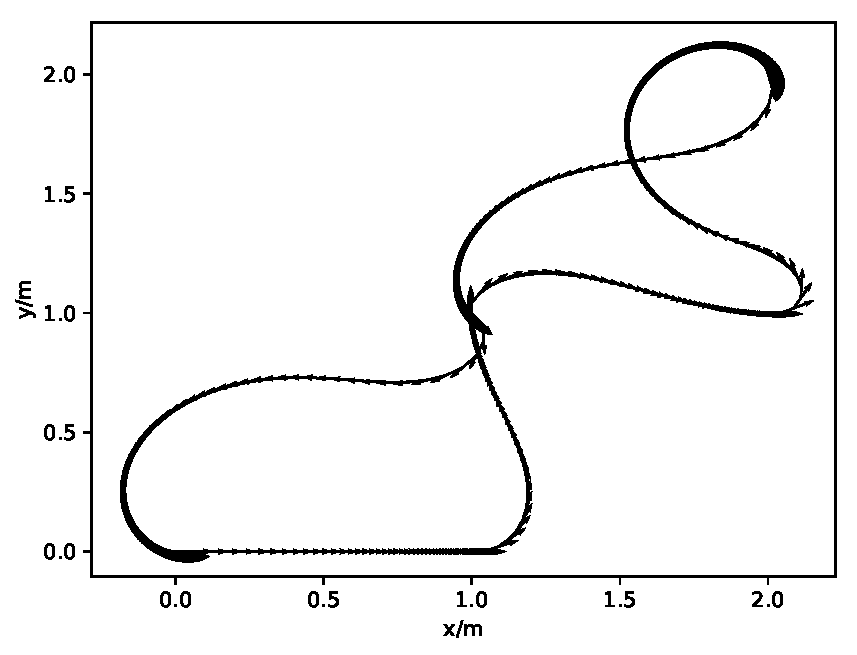
\includegraphics[width=0.7\textwidth]{../ideal_traj.pdf}
\caption{One generated trajectory.}\label{ideal}
\end{figure}
\section{Experiment and conclusion}
The algorithm is run on Sunfounder's PiCar-V platform with input \texttt{waypoints.txt}. The designed trajectory is shown as Fig.(\ref{act})

\begin{figure}[htbp]
\centering
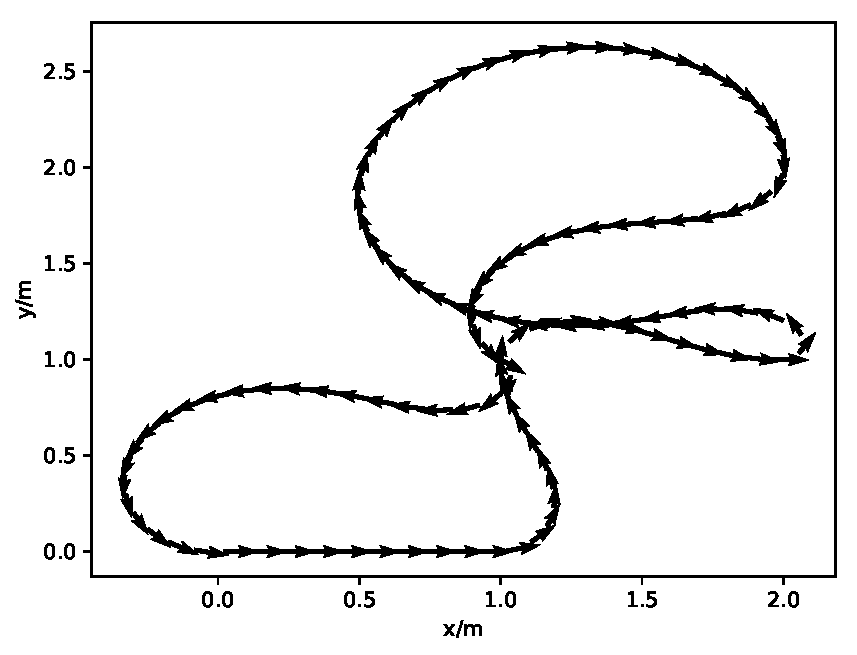
\includegraphics[width=0.7\textwidth]{../acutal_used.pdf}
\caption{The trajectory and control plan actually used.}\label{act}
\end{figure}

The error for each points is listed as Tab.(\ref{tab1}). The error-bar is given as the  95\% confidence interval.

\begin{table}[!h]
\centering
\caption{Experiment results on the robot}
\label{tab1}
\begin{tabular}{llr}

Waypoints   & $\Delta$ distance/m& $\Delta$ radian  \\
\hline
(0,0,0)        &/        &/\\
(1,0,0)      & $0.04 \pm 0.01$  &  $0.05 \pm 0.02$\\
(1,1,1.57)     &   $0.67 \pm 0.09$    & $0.70 \pm 0.12$\\
(2,1,0)  &    $0.86 \pm 0.10$    &  $0.32 \pm 0.04$\\
(2,2,-1.57)       &   $1.30 \pm 0.06$     &      $1.98 \pm 0.23$\\
(1,1,-.78)        &    $2.16 \pm 0.44$        &    $1.59 \pm 0.07$\\
(0.0.0)       &   $1.89 \pm 0.52$         &   $0.41 \pm 0.18$\\
\hline
\end{tabular}
\end{table}
It can be seen that the waypoint $(1,0,0)$ is the easiest and the algorithm can finish it almost without deviation. (1,1,1.57) and (1,1,-.78) are the two hardest: the former one requires a sharp turn and has high requirement for the pose estimation algorithm. The latter one contains continuous turning and again is hard for pose estimation.

The algorithm is able to drive the vehicle back (although with huge deviation) and has a relatively small deviation in terms of pose ($0.41$).

Clearly due to the lack of feedback, the error accumulates and the robot deviates more at the later waypoints. The robot is also prune to other issues such as motor acceleration rate, tyre pressure and turning rate limit, power difference of the two motors, etc. The algorithm, especially the pose estimation part does not accommodate the sliding and the road condition. Additionally, the control is over the motor power instead of the actual speed of the vehicle, which is the major source of uncertainty and error of the model.





%\begin{figure}[htbp]
%\centering
%\includegraphics[width=0.5\textwidth]{./src/lctwomethods.eps}
%\caption{Learning curve for steepest-direction coordinate descent and random-feature coordinate descent.}\label{fig1}
%\end{figure}

%\begin{table}[hp]
%\centering
%\caption{Experiment results}
%\label{tab1}
%\begin{tabular}{llr}
%
%$M$    & Prototype & Error rate (\%) \\
%\hline
%1000      & random    & $13.02 \pm  0.73$    \\
%          & random*        & $11. 84 \pm 0.20$      \\
%5000       & random     & $6.63 \pm 0.11$      \\
%		& random*     &$6.42 \pm 0.22$      \\
%10000       & random     & $5.07 \pm 0.2$     \\
%		 & random*      & $4.8 \pm 0.26$       \\
%\hline
%\end{tabular}
%\end{table}







%\subsection{Task 3}
%For 1000 different 100$\times$100 lattices with different $p$ values, the shortest path and the life time of fire is plotted in Fig.(\ref{fig3}). It can be seen clearly that the curves have a phase change point at $p_c\approx0.59$, after which the minimal step and life of fire drop quickly and approximates 100, the width of lattice.
%
%\begin{figure}[htbp]
%\centering
%\includegraphics[width=0.5\textwidth]{../figures/N100pvariable.eps}
%\caption{1000 different 100$\times$100 lattices with different $p$ values, the shortest path and the life time of fire}\label{fig3}
%\end{figure}
%
%For different values of width of lattice $N$, we use 1000 different random lattices per $N$ to find the correlation between the ratio of spanning cluster and the $p$ value, which is plotted in Fig.(\ref{fig4})
%
%
%\begin{figure}[htbp]
%\centering
%\includegraphics[width=0.5\textwidth]{../figures/ratio.eps}
%\caption{1000 different lattices of $N=50, 100, 200$ with different $p$ values, the ratio of the spanning cluster}\label{fig4}
%\end{figure}
%
%
%\section{Discussion}
%It can be found through these figures that $p_c\approx0.59$ and it is irrelevant to the width of lattice $N$.
%\begin{thebibliography}{99}
%
%\bibitem{knuth}
%  Knuth, Ervin D.,
%  \emph{The art of computer programming}, 
%  Addison Wesley, Massachusetts,
%  3rd edition,
%  1997.
%
%\end{thebibliography}

\end{document}